\documentclass[10pt,aspectratio=43]{beamer}

\usepackage{tikz}
\usepackage{xcolor}
\usepackage{caption}
\usepackage{subcaption}
\usepackage{bm}
\usetikzlibrary{calc} 
\usepackage{hyperref}
\hypersetup{
    colorlinks=true,
    linkcolor=blue,
    urlcolor=red
}
\usepackage{fontawesome5}

\usetheme{MyStyle}   % loads beamerthemeMyStyle.sty
\setlength{\columnsep}{0pt}


%%%%%%%%%%%%%%%%%%%%%%%%%%%%%%%%%%%%%%%%%%
%%%%%%%%%%%%%%%%%%%%%%%%%%%%%%%%%%%%%%%%%%
%%%%%%%%%%%%%%%%%%%%%%%%%%%%%%%%%%%%%%%%%%

\title{Kalman Filter updates}
\newcommand{\eventname}{ALERT meeting}
\author{Felix Touchte Codjo}
\institute{IJCLab}
\date{\today}


\begin{document}

\begin{frame}[plain] % remove header, footer, barre de navigation
\titlepage
\end{frame}

%\begin{frame}{Outline}
%\tableofcontents
%\end{frame}

%\section{Intro}
\section{Updates}
\begin{frame}{Updates - AHDC alignement}
    \begin{itemize}
        \item Procedure:
            \begin{enumerate}
                \item We looked at elastic events : electron + track (here: collection of hits only)
                \item We computed the theoretical momentum vector of the track $\vec{p}$
                \item We made the propagation without doing any fit (i.e no KF correction)
                \item We looked at {\color{blue} residual\_LR} (left-right) $\longrightarrow$ sensitive to the alignment
            \end{enumerate}
    \end{itemize}
    

    \vspace{0.2cm}
    \centering
    \begin{minipage}{0.5\textwidth}
        \includegraphics[width=\linewidth]{figures/build/illustration_residual_type.pdf}
    \end{minipage}

\end{frame}

\begin{frame}{Updates - AHDC alignement}
    \begin{itemize}
        \item Residual LR with no alignment (no fit)
        \item Even layer number need to be rotated to the phi $+$
    \end{itemize}

    \vspace{0.2cm}
    \centering
    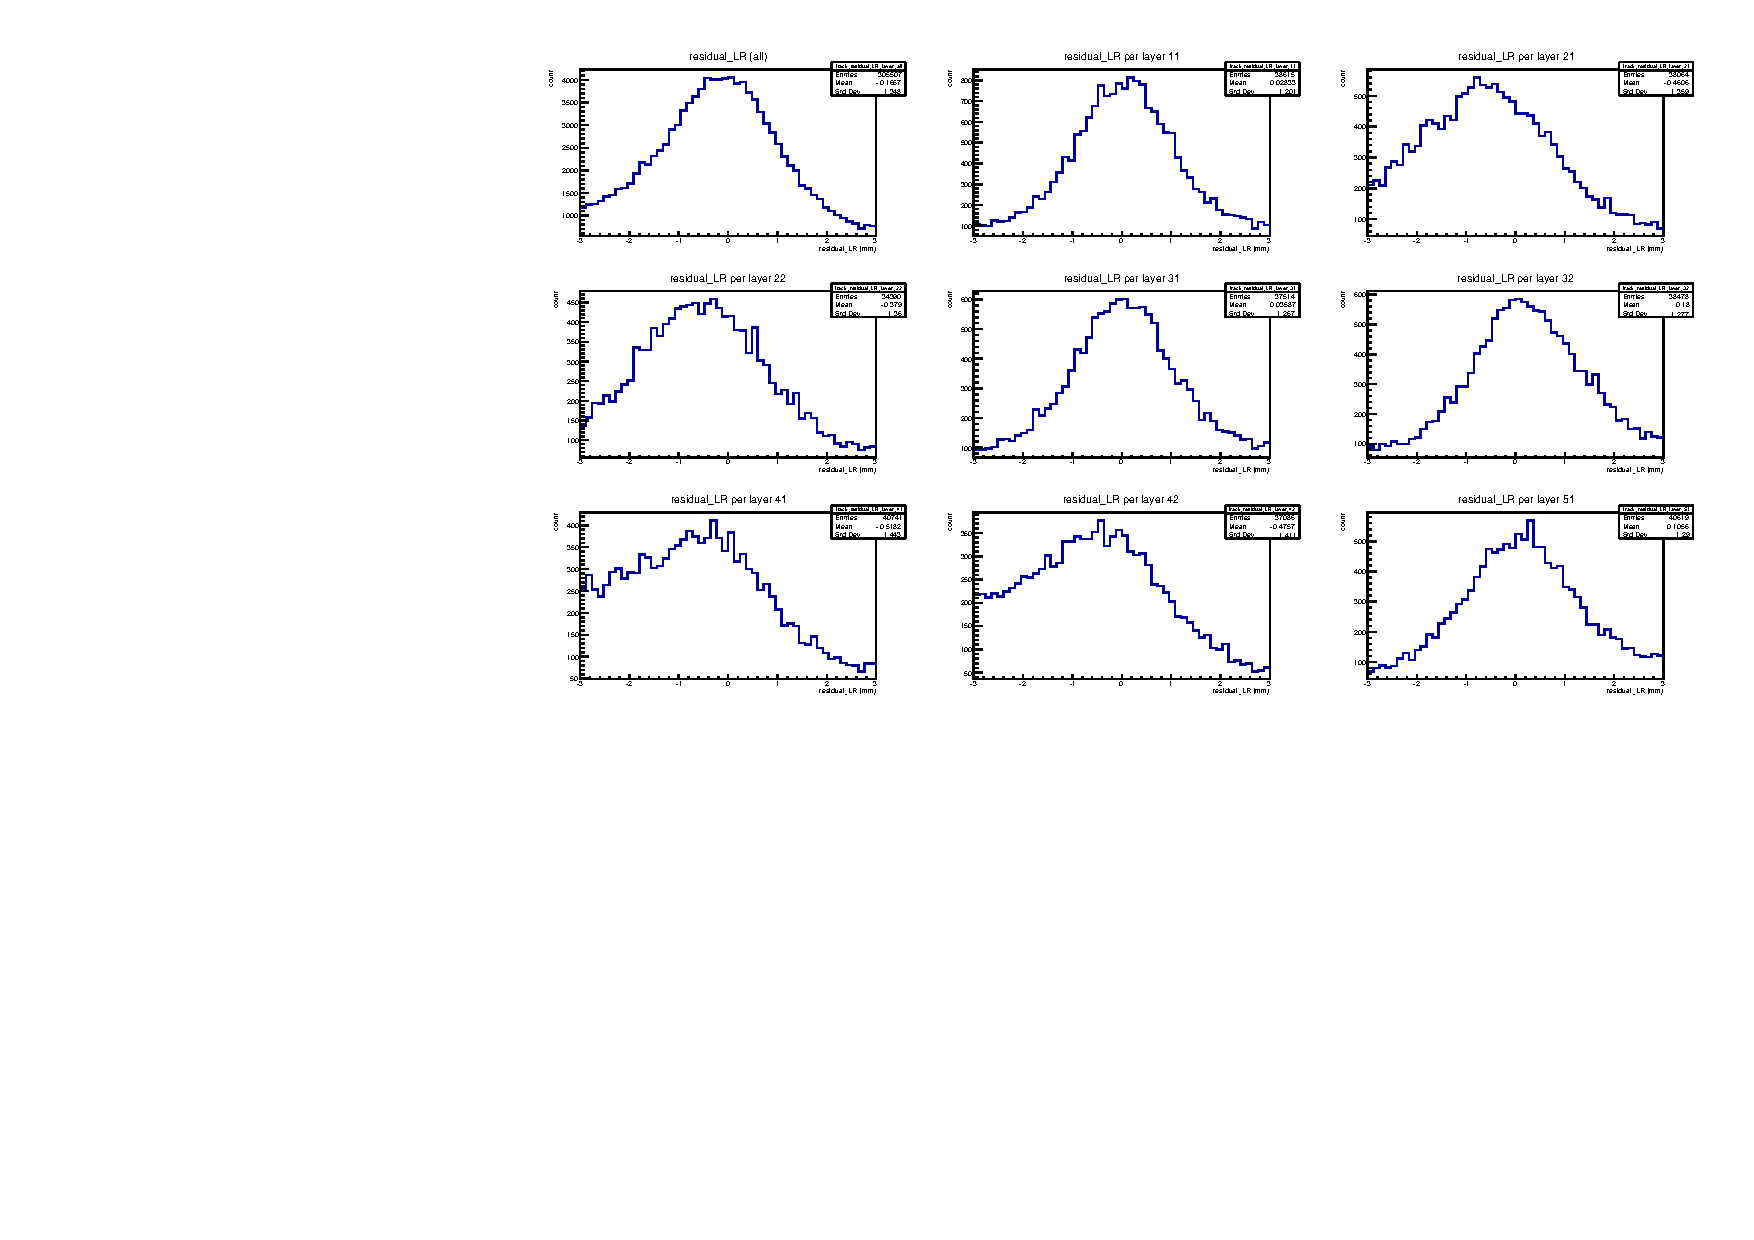
\includegraphics[width=0.9\textwidth]{figures/residual_LR_v109_no_alignment.pdf}

\end{frame}

\begin{frame}{Updates - AHDC alignement}
    \begin{itemize}
        \item Residual LR after \textbf{layer alignment} (first attempt, but few iterations) (no fit)
        \item RotationZ: 0$^\circ$, +2.55$^\circ$, +2.11$^\circ$, 0$^\circ$, -0.32$^\circ$, +2.37$^\circ$, +2.13$^\circ$, -0.21$^\circ$
    \end{itemize}

    \vspace{0.2cm}
    \centering
    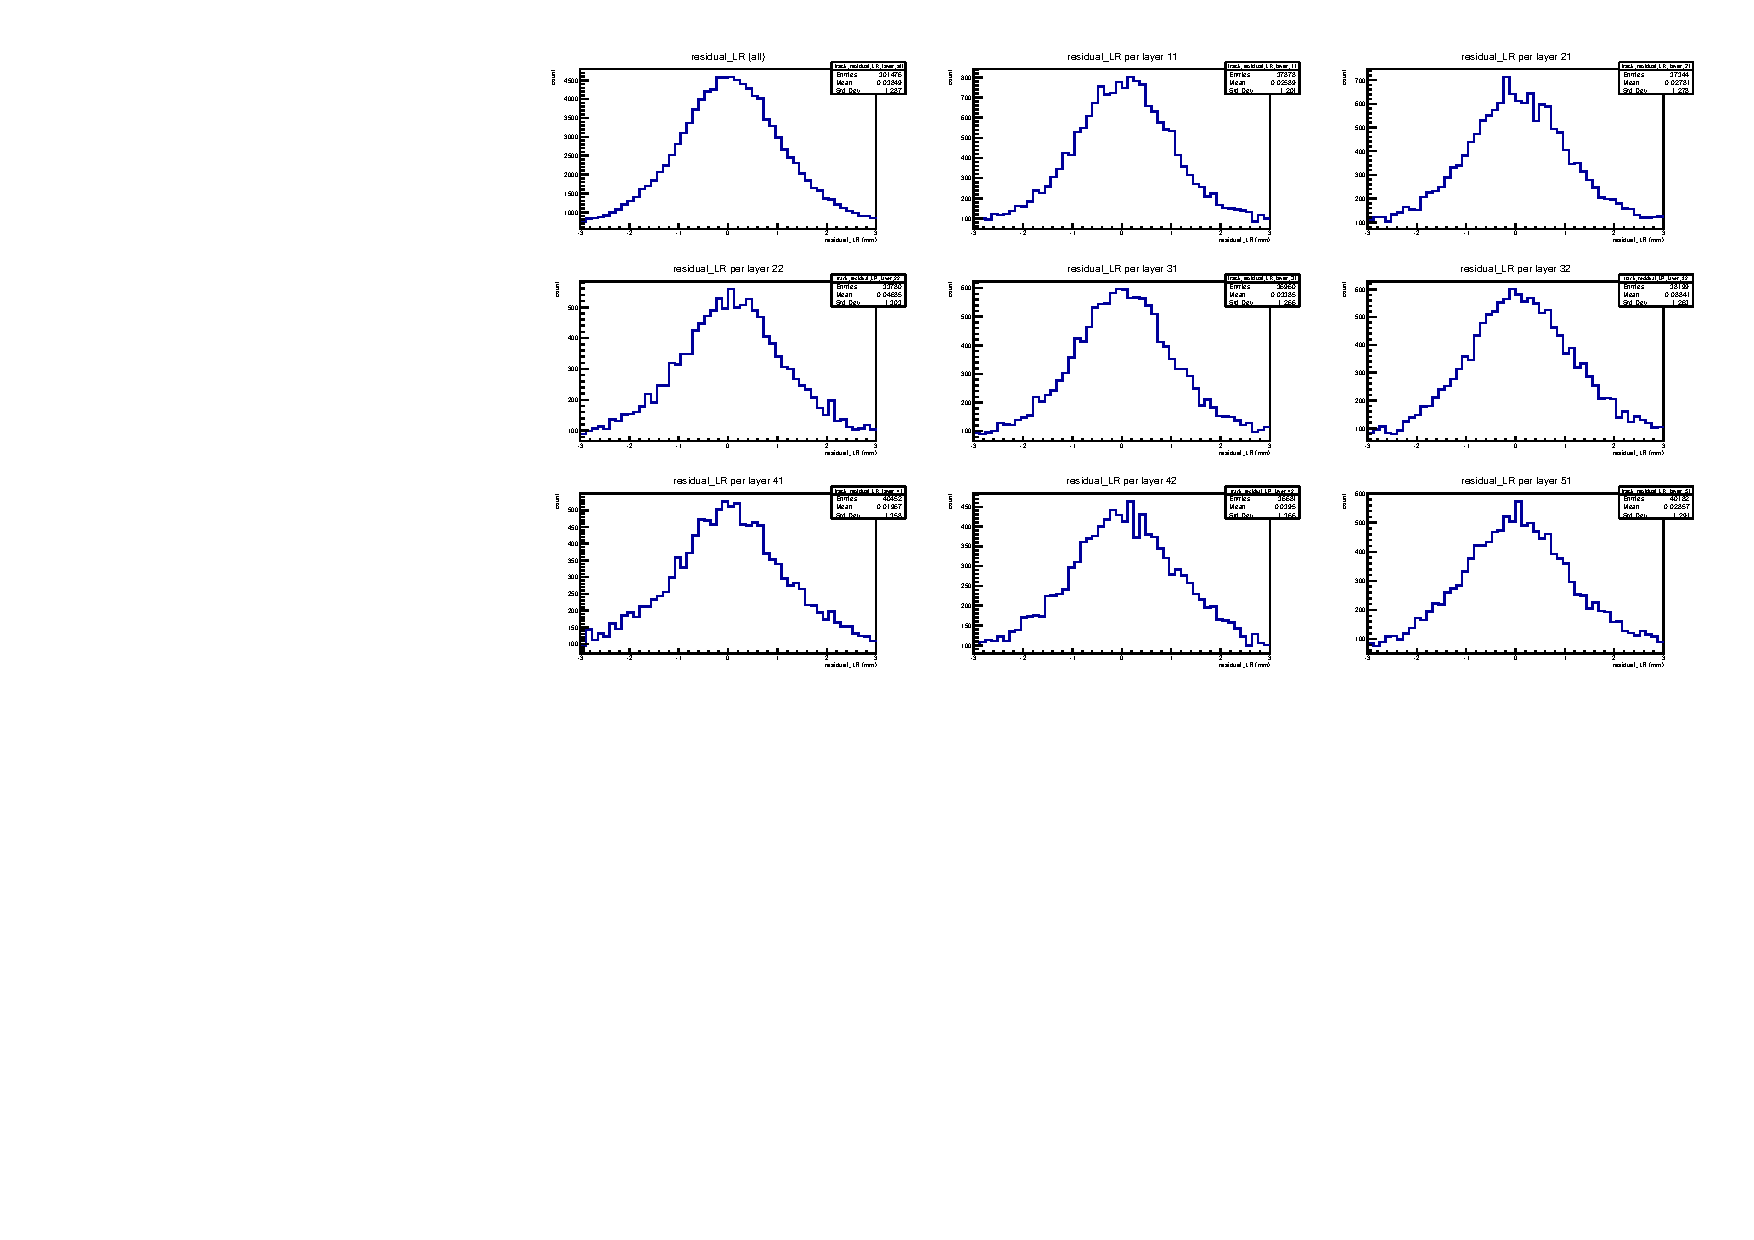
\includegraphics[width=0.9\textwidth]{figures/residual_LR_v113_with_alignment.pdf}

\end{frame}

\begin{frame}{Updates - AHDC alignement}
    \begin{itemize}
        \item Effect on theta (when we run the Kalman Filter fit)
        \item The {\color{blue} residual\_LR} is a good observable for the AHDC alignment
    \end{itemize}

    \vspace{0.5cm}
    \centering

    \begin{minipage}{0.45\textwidth}
        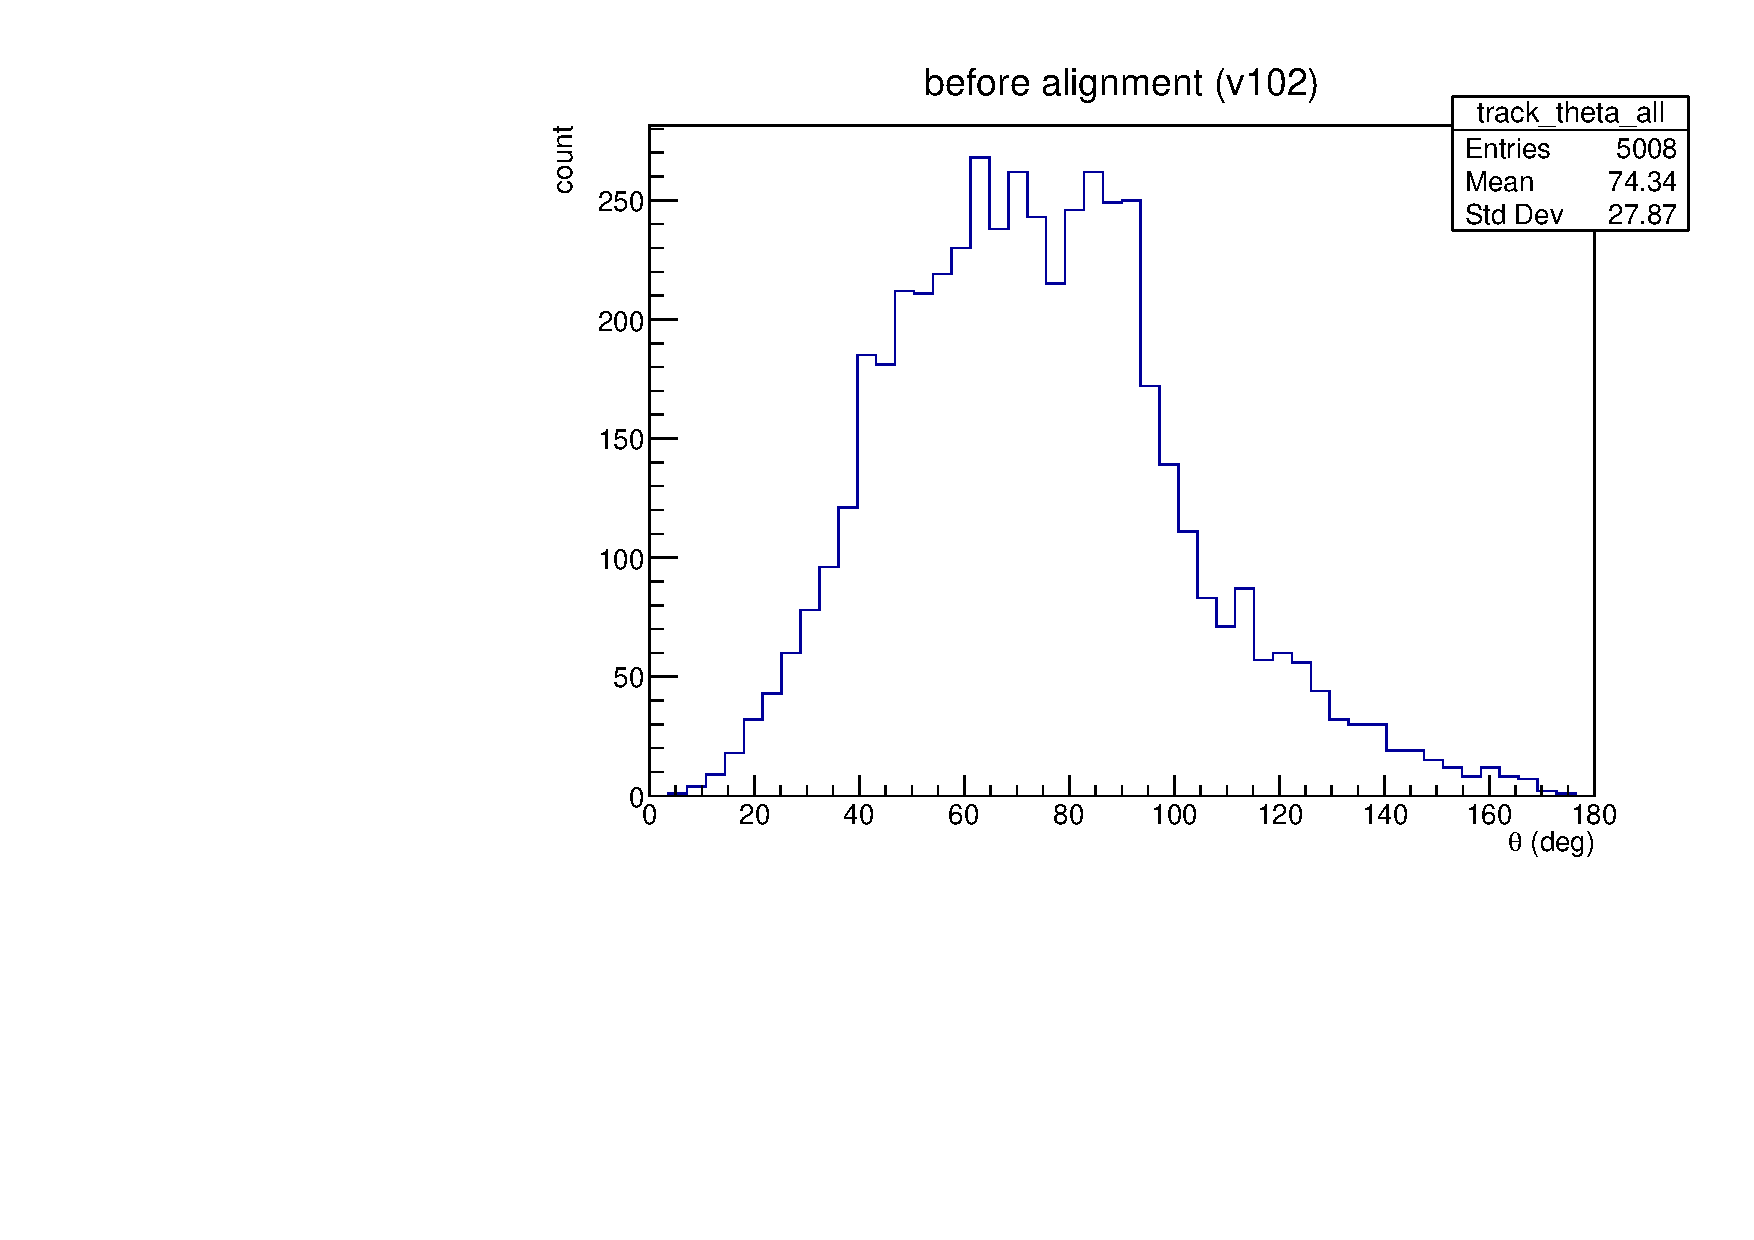
\includegraphics[width=\linewidth]{figures/theta_no_alignment_v102.pdf}
    \end{minipage}
    \begin{minipage}{0.45\textwidth}
        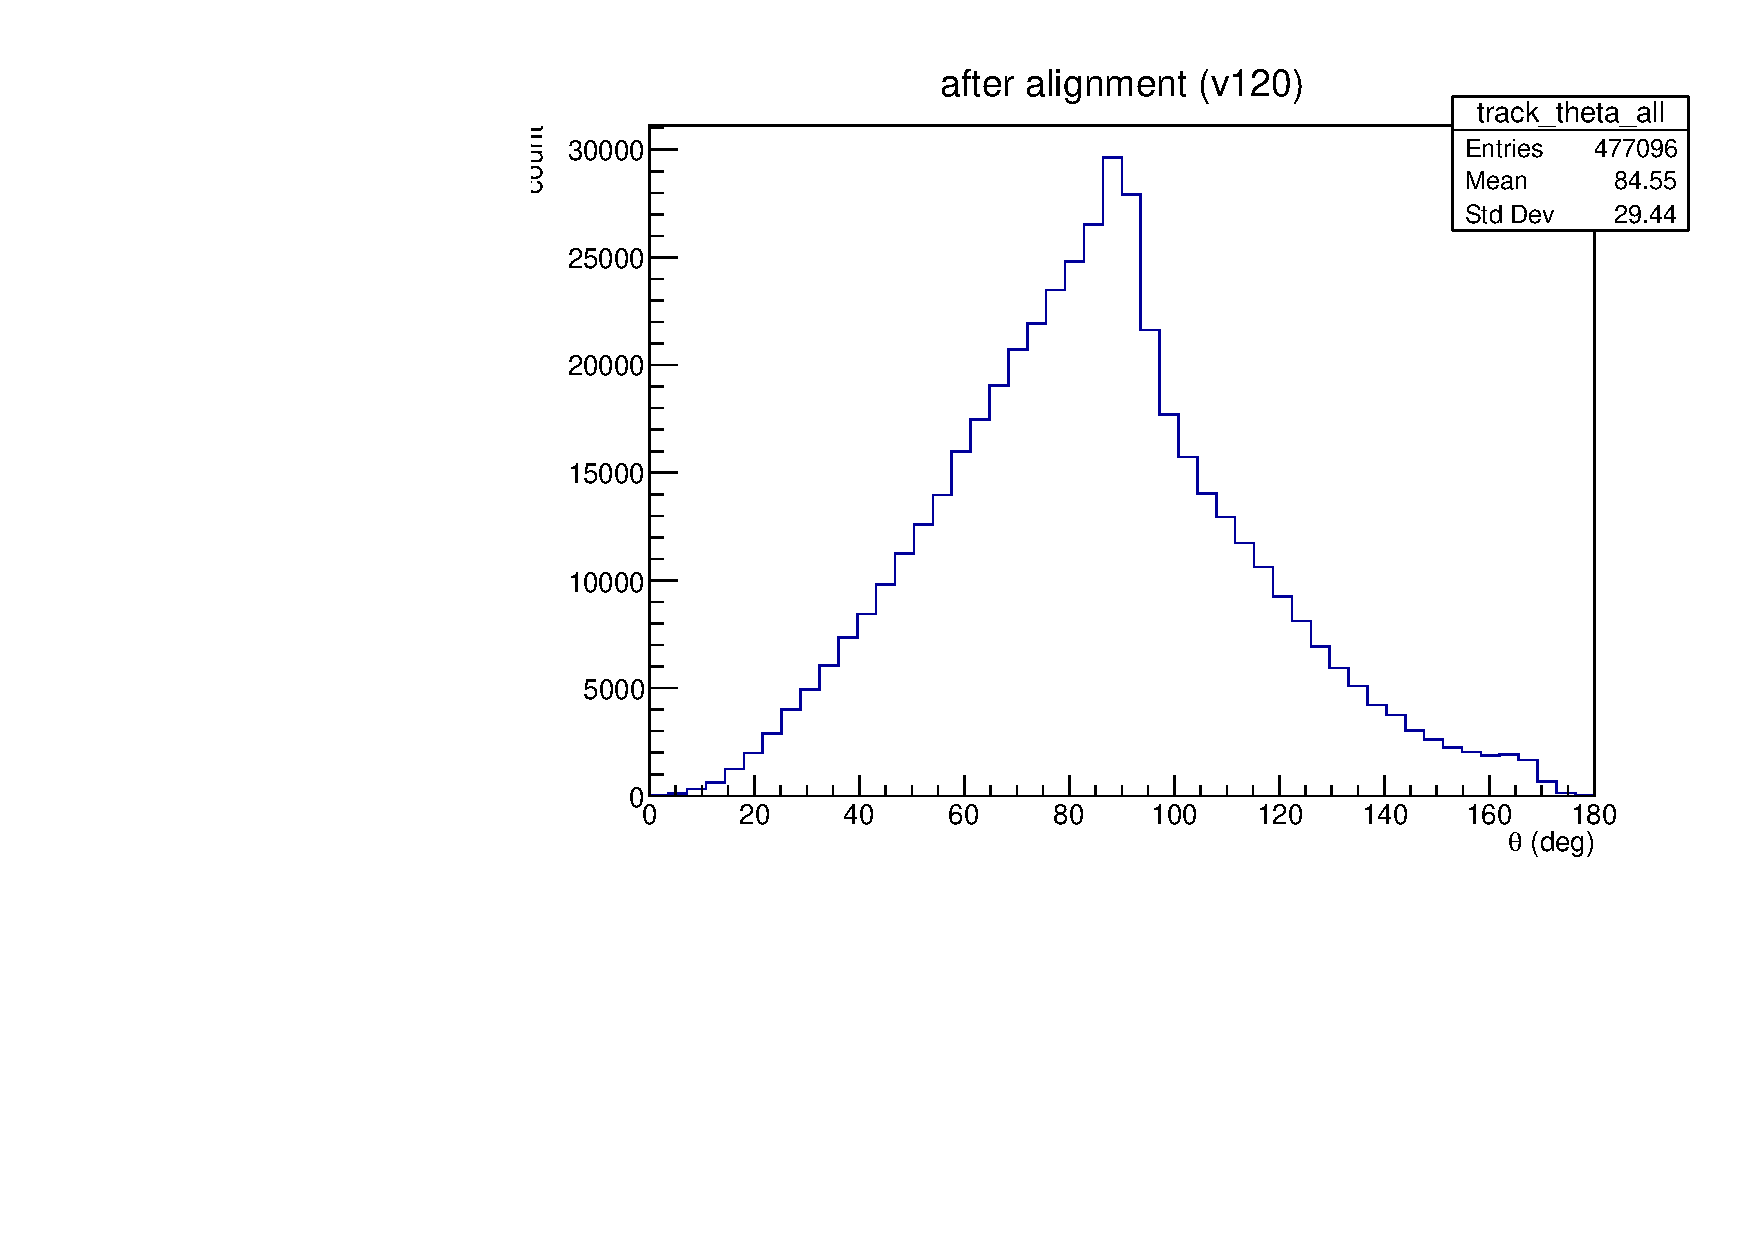
\includegraphics[width=\linewidth]{figures/theta_with_alignment_v120.pdf}
    \end{minipage}
\end{frame}

\begin{frame}{Updates - AHDC alignement}
    \begin{itemize}
        \item Layer by layer residual after the fit
        \item After the fit, the last layer get misalign
    \end{itemize}

    \vspace{0.2cm}
    \centering

    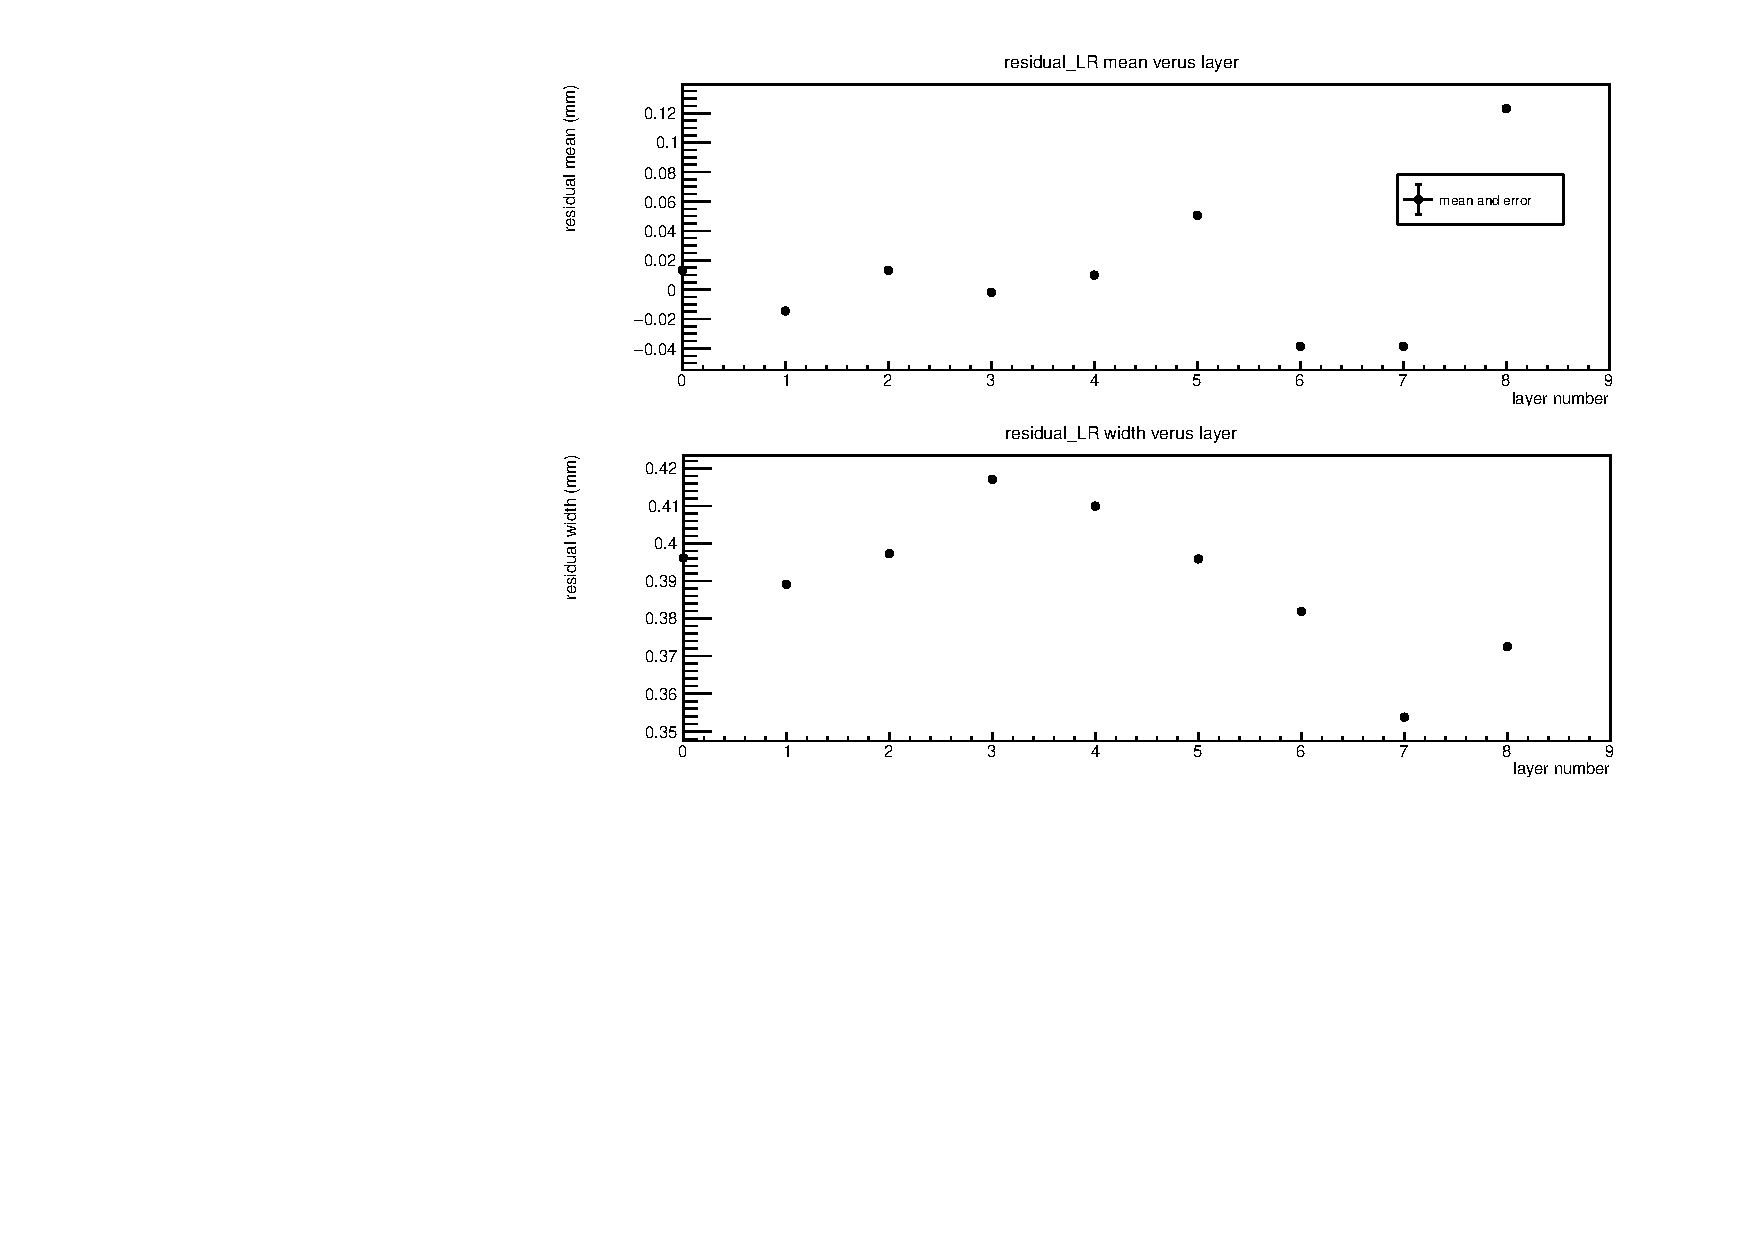
\includegraphics[width=0.9\textwidth]{figures/residual_per_layer.pdf}

\end{frame}

\begin{frame}{Updates - AHDC alignement}
    \begin{itemize}
        \item We may need to look wire by wire (the fit is done)
    \end{itemize}

    \vspace{0.2cm}
    \centering

    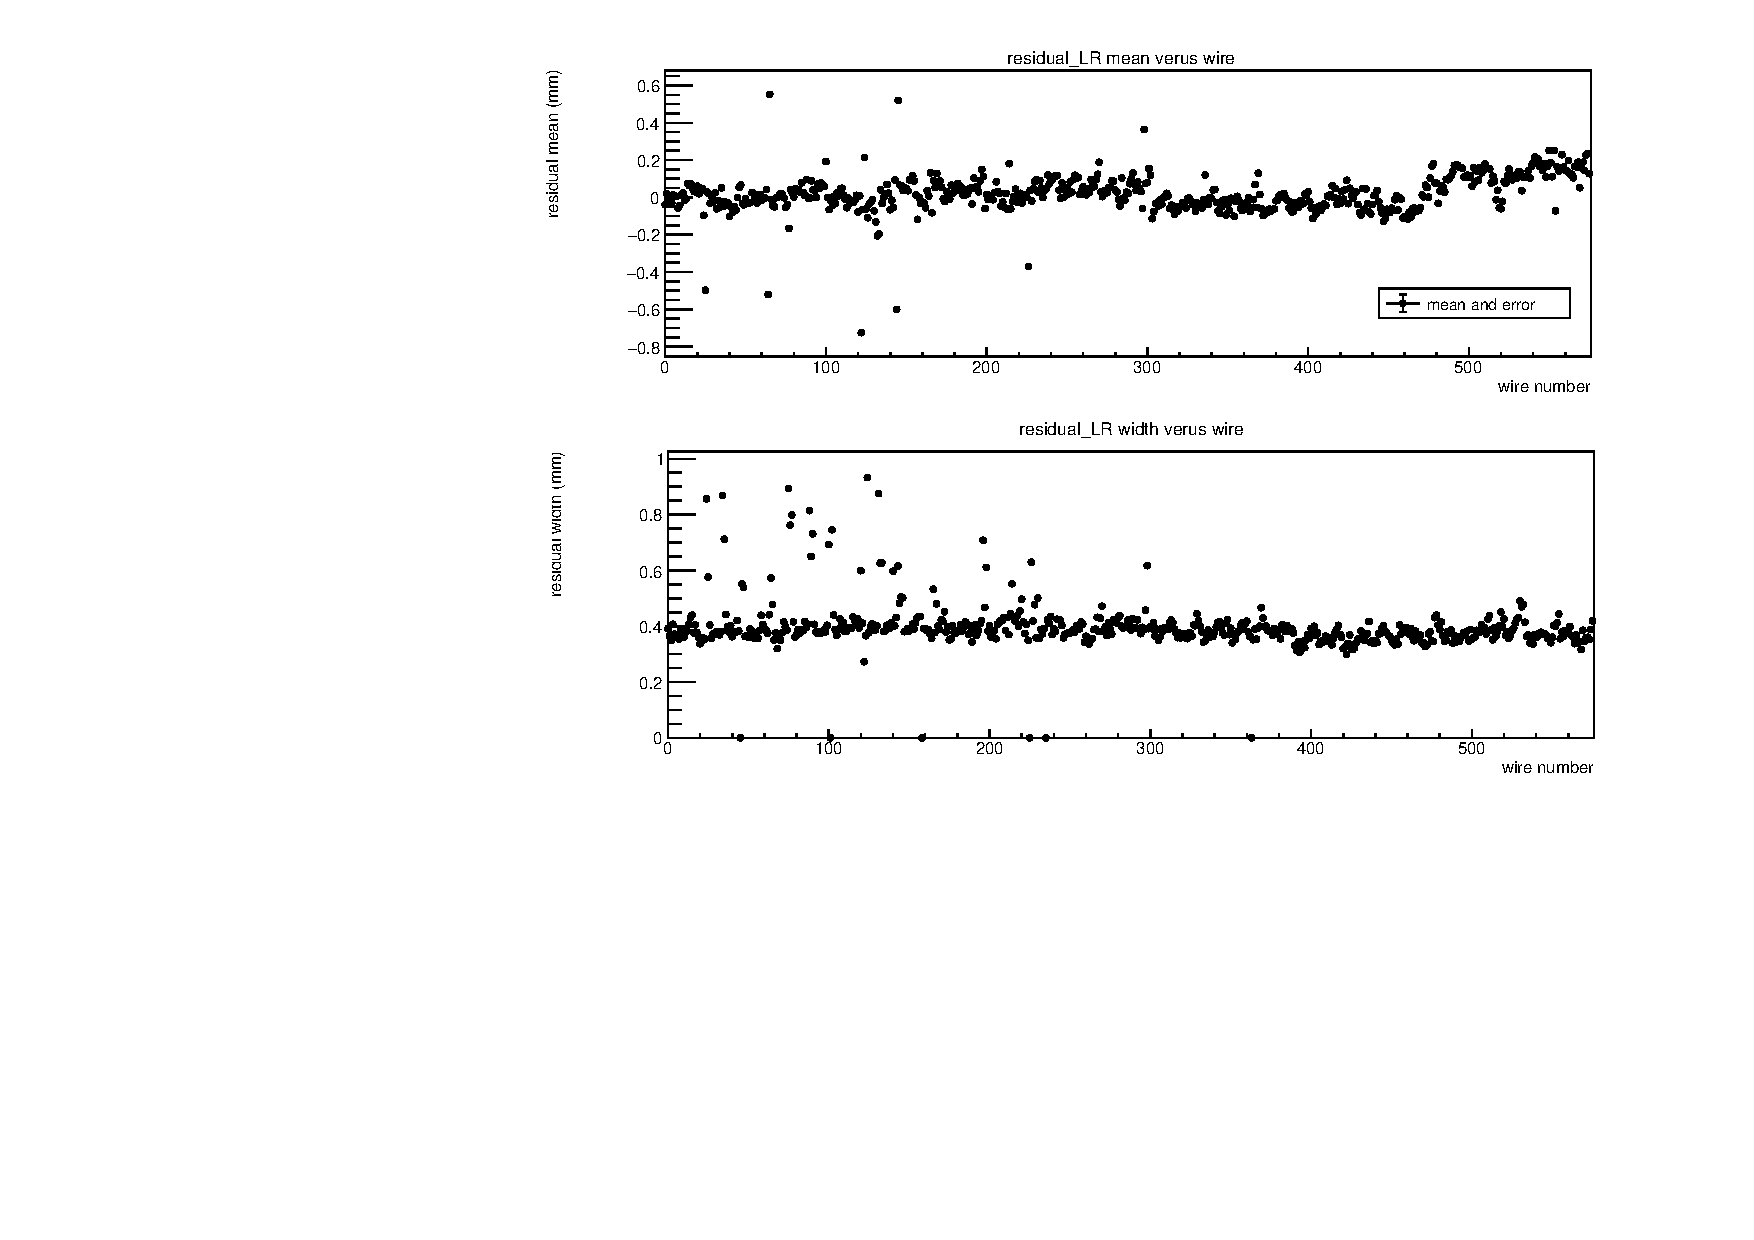
\includegraphics[width=0.9\textwidth]{figures/residual_per_wire.pdf}

\end{frame}

\begin{frame}{Updates - AHDC alignement}
    \begin{itemize}
        \item We may also have a vz dependence (the fit is done)
        %\item The fit is done
    \end{itemize}

    \vspace{0.2cm}
    \centering

    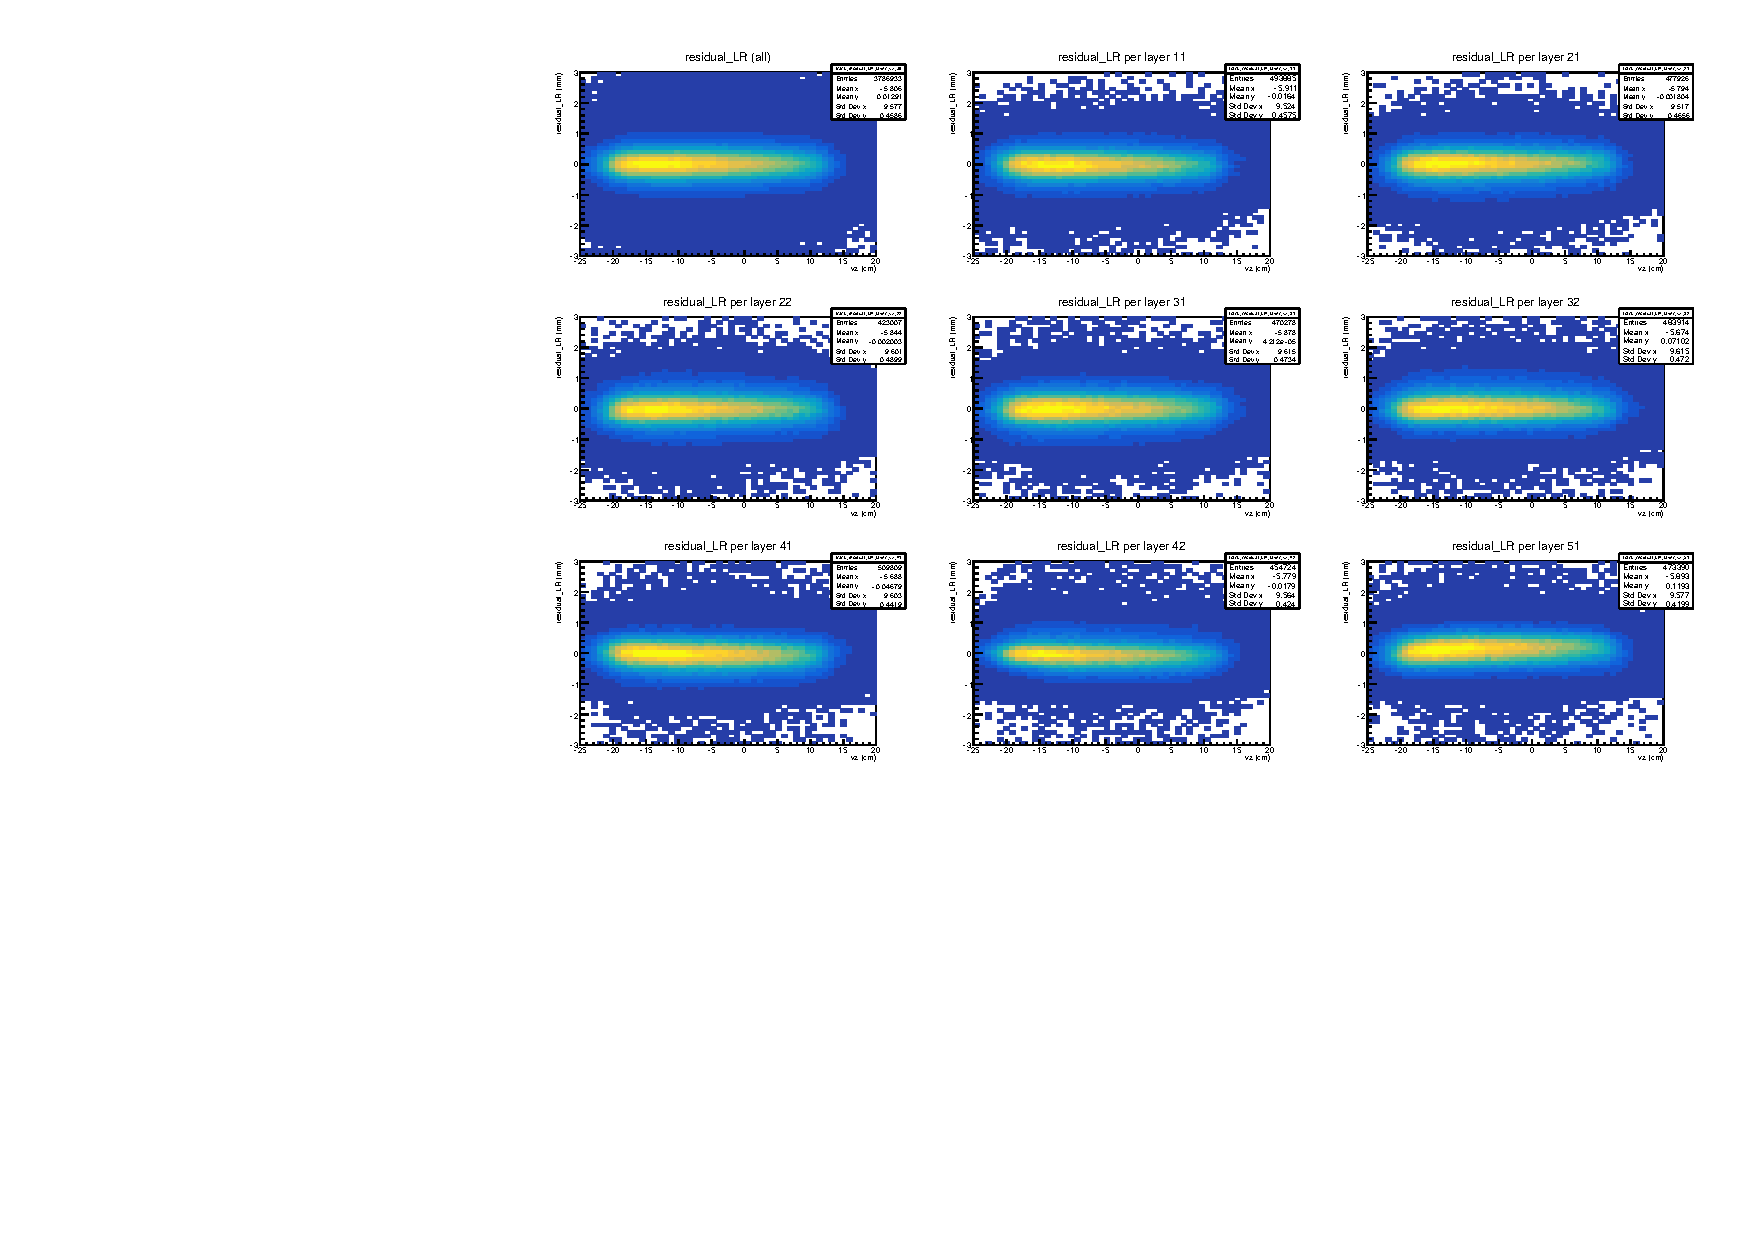
\includegraphics[width=0.9\textwidth]{figures/residual_2D_per_layer.pdf}

\end{frame}

% \begin{frame}{ATOF hit work completed 2/2}
%     \begin{itemize}
%         \item Status of the theta reconstruction
%         \item We have two peaks in the last version of the theta reconstruction
%             \begin{itemize}
%                 \item The first peak are tracks without ATOF matches
%                 \item The second peak around 86$^\circ$ are tracks with ATOF matches (45 \%)
%             \end{itemize}
%         \item The final 45 \% matches (over the nb. tracks) is low; it is essentially due the current misalignment between the AHDC and ATOF
%     \end{itemize}

%     \vspace{0.5cm}

%     \centering
%     \begin{minipage}{0.32\textwidth}
%         
\includegraphics[width=\linewidth]{figures/data_theta_new_geometry.pdf}
%     \end{minipage}
%     \begin{minipage}{0.32\textwidth}
%         
\includegraphics[width=\linewidth]{figures/data_theta_ai_matching.pdf}
%     \end{minipage}
%     \begin{minipage}{0.32\textwidth}
%         
\includegraphics[width=\linewidth]{figures/data_theta_proj_based_matching.pdf}
%     \end{minipage}

% \end{frame}

% \section{Next steps}
% \begin{frame}{Next steps}
%     \begin{itemize}
%         \item Convenient use of the PID
%             \begin{itemize}
%                 \item For now, the energy loss and the curvature assume the particle to be a proton
%                 \item We will use the PrePID work of Uditha \href{https://indico.jlab.org/event/1017/\#73-alert-ai-particle-identific}{(\underline{link}) {\scriptsize \faExternalLink*}}
%             \end{itemize}
%         \item Material verification
%             \begin{itemize}
%                 \item Correct density for the target straw, target gas, ATOF scintillator
%                 \item Correct use in the Kalman Filter propagator
%                 \item \textbf{Vary the density of the target gas with the temperature and the pressure condition over the run period}
%             \end{itemize}
%         \item Fine-tuning
%             \begin{itemize}
%                 \item Electron vertex resolution on $p_e$ and $\theta_e$
%                 \item Measurement noise of the AHDC hits (ADC and time dependence)
%                 \item ATOF hits resolution for clusters
%                 \item Initial error covariance matrix
%             \end{itemize}
%         \item Work on the AHDC alignment
%             \begin{itemize}
%                 \item With respect to CLAS
%                 \item With respect to ATOF
%             \end{itemize}
%     \end{itemize}

%     %\vspace{0.5cm}

% \end{frame}






\end{document}


